% !TeX program = xelatex
\documentclass[12pt, a4paper]{article}
\usepackage{amsmath}
\usepackage{xeCJK}
\usepackage{amsmath}
\usepackage{amssymb}
\usepackage{parskip}
\usepackage{tikz}
\usepackage{enumitem}

\setmainfont{Latin Modern Roman}
\setCJKmainfont{Noto Serif CJK TC}

\title{Stable Current}

\begin{document}
\section*{Resistance Calculations}
\begin{center}


\tikzset{every picture/.style={line width=0.75pt}} %set default line width to 0.75pt        

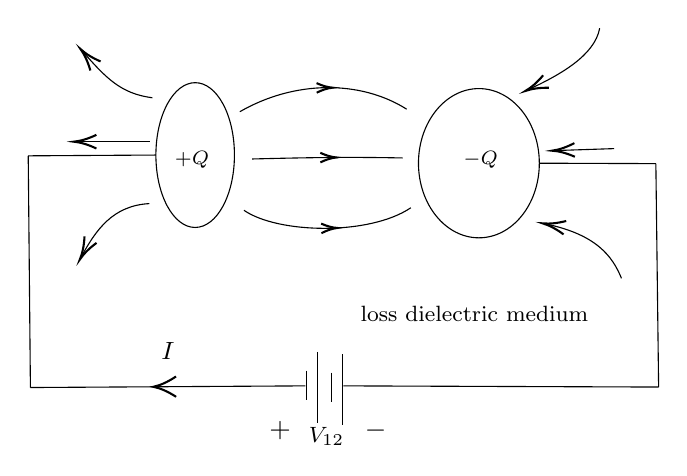
\begin{tikzpicture}[x=0.75pt,y=0.75pt,yscale=-1,xscale=1]
%uncomment if require: \path (0,300); %set diagram left start at 0, and has height of 300

%Shape: Ellipse [id:dp4009139407527874] 
\draw   (253.23,47.35) .. controls (269.31,47.35) and (282.34,63.45) .. (282.34,83.3) .. controls (282.34,103.15) and (269.31,119.25) .. (253.23,119.25) .. controls (237.16,119.25) and (224.12,103.15) .. (224.12,83.3) .. controls (224.12,63.45) and (237.16,47.35) .. (253.23,47.35) -- cycle ;
%Shape: Ellipse [id:dp9736259016812426] 
\draw   (116.55,44.5) .. controls (127,44.5) and (135.46,60.12) .. (135.45,79.39) .. controls (135.44,98.65) and (126.96,114.26) .. (116.51,114.26) .. controls (106.06,114.25) and (97.6,98.63) .. (97.61,79.37) .. controls (97.62,60.11) and (106.1,44.49) .. (116.55,44.5) -- cycle ;
%Curve Lines [id:da24459020107782226] 
\draw    (138.05,58.5) .. controls (164.43,43.27) and (196.13,43.18) .. (218.43,57.27) ;
\draw [shift={(182.7,46.91)}, rotate = 179.18] [color={rgb, 255:red, 0; green, 0; blue, 0 }  ][line width=0.75]    (7.65,-2.3) .. controls (4.86,-0.97) and (2.31,-0.21) .. (0,0) .. controls (2.31,0.21) and (4.86,0.98) .. (7.65,2.3)   ;
%Curve Lines [id:da9462490695524745] 
\draw    (143.93,81.27) .. controls (172.81,80.53) and (190.93,80.27) .. (216.43,80.77) ;
\draw [shift={(184.5,80.53)}, rotate = 179.52] [color={rgb, 255:red, 0; green, 0; blue, 0 }  ][line width=0.75]    (7.65,-2.3) .. controls (4.86,-0.97) and (2.31,-0.21) .. (0,0) .. controls (2.31,0.21) and (4.86,0.98) .. (7.65,2.3)   ;
%Curve Lines [id:da1296882326892388] 
\draw    (140.05,106) .. controls (156.43,117.27) and (200.43,118.27) .. (220.43,104.77) ;
\draw [shift={(184.96,114.5)}, rotate = 178.4] [color={rgb, 255:red, 0; green, 0; blue, 0 }  ][line width=0.75]    (7.65,-2.3) .. controls (4.86,-0.97) and (2.31,-0.21) .. (0,0) .. controls (2.31,0.21) and (4.86,0.98) .. (7.65,2.3)   ;
%Curve Lines [id:da015162286974555239] 
\draw    (311.43,18.27) .. controls (309.02,31.29) and (292.64,40.6) .. (277.28,47.73) ;
\draw [shift={(275.61,48.5)}, rotate = 335.43] [color={rgb, 255:red, 0; green, 0; blue, 0 }  ][line width=0.75]    (10.93,-3.29) .. controls (6.95,-1.4) and (3.31,-0.3) .. (0,0) .. controls (3.31,0.3) and (6.95,1.4) .. (10.93,3.29)   ;
%Straight Lines [id:da6191094576803734] 
\draw    (318.43,76.27) -- (290.43,77.2) ;
\draw [shift={(288.43,77.27)}, rotate = 358.09] [color={rgb, 255:red, 0; green, 0; blue, 0 }  ][line width=0.75]    (10.93,-3.29) .. controls (6.95,-1.4) and (3.31,-0.3) .. (0,0) .. controls (3.31,0.3) and (6.95,1.4) .. (10.93,3.29)   ;
%Curve Lines [id:da8380778513317244] 
\draw    (321.93,138.77) .. controls (317.54,128.04) and (309.83,117.79) .. (285.81,112.65) ;
\draw [shift={(283.93,112.27)}, rotate = 11.09] [color={rgb, 255:red, 0; green, 0; blue, 0 }  ][line width=0.75]    (10.93,-3.29) .. controls (6.95,-1.4) and (3.31,-0.3) .. (0,0) .. controls (3.31,0.3) and (6.95,1.4) .. (10.93,3.29)   ;
%Curve Lines [id:da054493417925754684] 
\draw    (95.93,51.77) .. controls (80.49,49.84) and (73.27,41.85) .. (62.45,29.61) ;
\draw [shift={(61.26,28.27)}, rotate = 48.5] [color={rgb, 255:red, 0; green, 0; blue, 0 }  ][line width=0.75]    (10.93,-3.29) .. controls (6.95,-1.4) and (3.31,-0.3) .. (0,0) .. controls (3.31,0.3) and (6.95,1.4) .. (10.93,3.29)   ;
%Straight Lines [id:da4305209594574675] 
\draw    (94.6,72.93) -- (60.01,72.93) ;
\draw [shift={(58.01,72.93)}, rotate = 360] [color={rgb, 255:red, 0; green, 0; blue, 0 }  ][line width=0.75]    (10.93,-3.29) .. controls (6.95,-1.4) and (3.31,-0.3) .. (0,0) .. controls (3.31,0.3) and (6.95,1.4) .. (10.93,3.29)   ;
%Curve Lines [id:da8167888171914996] 
\draw    (94.43,102.77) .. controls (76.76,103.72) and (68.67,115.62) .. (61.88,128.01) ;
\draw [shift={(60.93,129.77)}, rotate = 298.3] [color={rgb, 255:red, 0; green, 0; blue, 0 }  ][line width=0.75]    (10.93,-3.29) .. controls (6.95,-1.4) and (3.31,-0.3) .. (0,0) .. controls (3.31,0.3) and (6.95,1.4) .. (10.93,3.29)   ;
%Straight Lines [id:da5463097272385813] 
\draw    (97.61,79.37) -- (36.1,79.75) ;
%Straight Lines [id:da6618446595905129] 
\draw    (37.15,191.38) -- (36.1,79.75) ;
%Straight Lines [id:da049513316176787336] 
\draw    (339.82,191.15) -- (338.49,83.5) ;
%Straight Lines [id:da3790801442577336] 
\draw    (338.49,83.5) -- (282.34,83.3) ;

%Straight Lines [id:da8984791750560811] 
\draw    (37.15,191.38) -- (169.66,190.58) ;
\draw [shift={(96.41,191.03)}, rotate = 359.65] [color={rgb, 255:red, 0; green, 0; blue, 0 }  ][line width=0.75]    (10.93,-4.9) .. controls (6.95,-2.3) and (3.31,-0.67) .. (0,0) .. controls (3.31,0.67) and (6.95,2.3) .. (10.93,4.9)   ;
%Straight Lines [id:da6465607542782179] 
\draw    (187.9,190.58) -- (339.82,191.15) ;
%Straight Lines [id:da4118347597147364] 
\draw    (170.23,183.25) -- (170.23,197.25) ;
%Straight Lines [id:da7814164919371904] 
\draw    (175.56,174.25) -- (175.56,208.58) ;
%Straight Lines [id:da41666702605710226] 
\draw    (182.23,184.25) -- (182.23,198.25) ;
%Straight Lines [id:da7009304855314259] 
\draw    (187.56,175.25) -- (187.56,209.58) ;

% Text Node
\draw (105.52,76.4) node [anchor=north west][inner sep=0.75pt]  [font=\scriptsize]  {$+Q$};
% Text Node
\draw (244.52,76.4) node [anchor=north west][inner sep=0.75pt]  [font=\scriptsize]  {$-Q$};
% Text Node
\draw (99,168.4) node [anchor=north west][inner sep=0.75pt]  [font=\small]  {$I$};
% Text Node
\draw (151,206.4) node [anchor=north west][inner sep=0.75pt]    {$+$};
% Text Node
\draw (197,206.4) node [anchor=north west][inner sep=0.75pt]    {$-$};
% Text Node
\draw (170,209.4) node [anchor=north west][inner sep=0.75pt]  [font=\footnotesize]  {$V_{12}$};
% Text Node
\draw (195,151) node [anchor=north west][inner sep=0.75pt]  [font=\footnotesize] [align=left] {loss dielectric medium};
\end{tikzpicture}
\end{center}

$$
RC = \frac{\epsilon}{\sigma}
$$
We can prove that by $C = \frac{Q}{V}$ and $R = \frac{V}{I}$
\begin{align*}
	C &= \frac{Q}{V} = \frac{\oint_s \vec D \cdot \text{d} \vec s}{-\int \vec E \cdot \text{d} \vec l} = \frac{\oint_s \epsilon \vec E \cdot \text{d} \vec s}{-\int_L \vec E \cdot \text{d} \vec l} \\ \\
	R &= \frac{V}{I} = \frac{-\int_L \vec E \cdot \text{d} \vec l}{\oint_s \vec J \cdot \text{d} \vec s} = \frac{-\int_L \vec E \cdot \text{d} \vec l}{\oint_s \sigma \vec E \cdot \text{d} \vec s} \\ \\
	RC &= \frac{-\int_L \vec E \cdot \text{d} \vec l}{\sigma \oint_s \vec E \cdot \text{d} \vec s} \cdot \frac{\epsilon \oint_s \vec E \cdot \text{d} \vec l}{-\int_L \vec E \cdot \text{d} \vec l} = \frac{\epsilon}{\sigma}
\end{align*}

\begin{enumerate}[label=\arabic*:]
	\item appropriate coordinate
	\item $V_0$ (potential difference between conductor terminals)
	\item $\vec E$ = ? homogeneous (constant conductivity)
	\item $I = \int_s \vec J \cdot \text{d} \vec s = \int_s \sigma \vec E \cdot \text{d} \vec s$
	\item $R = \frac{V_0}{I}$
\end{enumerate}
\newpage

\textbf{Exercise 4-4} \\
一個均勻厚度為$h$,導電率$\sigma$的導電材料具有一個扁平的環形墊圈的1/4的形狀,其內徑為$a$,外徑為$b$,如下圖所示。決定在二端點面間的電阻。 
\begin{center}


\tikzset{every picture/.style={line width=0.75pt}} %set default line width to 0.75pt        

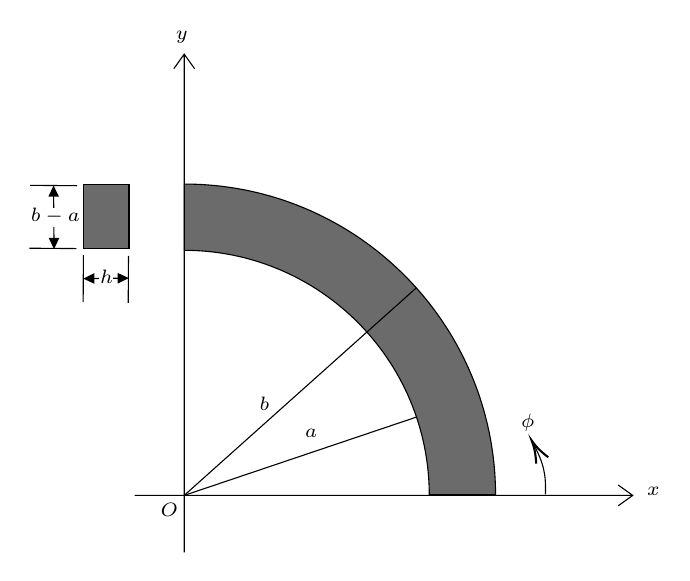
\begin{tikzpicture}[x=0.75pt,y=0.75pt,yscale=-1,xscale=1]
%uncomment if require: \path (0,300); %set diagram left start at 0, and has height of 300

%Shape: Axis 2D [id:dp8619576860094512] 
\draw  (292.56,243.57) -- (532.56,243.57)(316.46,31) -- (316.46,271) (525.56,238.57) -- (532.56,243.57) -- (525.56,248.57) (311.46,38) -- (316.46,31) -- (321.46,38)  ;
%Shape: Block Arc [id:dp9979602959498808] 
\draw  [fill={rgb, 255:red, 0; green, 0; blue, 0 }  ,fill opacity=0.58 ] (316.56,93.57) .. controls (399.23,93.62) and (466.24,160.55) .. (466.46,243.17) -- (434.53,243.26) .. controls (434.36,178.22) and (381.61,125.54) .. (316.54,125.49) -- cycle ;
%Shape: Rectangle [id:dp33966397929339964] 
\draw  [fill={rgb, 255:red, 0; green, 0; blue, 0 }  ,fill opacity=0.58 ] (267.86,93.92) -- (289.87,93.92) -- (289.87,124.83) -- (267.86,124.83) -- cycle ;
%Straight Lines [id:da5405684515583616] 
\draw    (270.83,139.1) -- (286.77,138.92) ;
\draw [shift={(289.77,138.88)}, rotate = 179.34] [fill={rgb, 255:red, 0; green, 0; blue, 0 }  ][line width=0.08]  [draw opacity=0] (5.36,-2.57) -- (0,0) -- (5.36,2.57) -- cycle    ;
\draw [shift={(267.83,139.13)}, rotate = 359.34] [fill={rgb, 255:red, 0; green, 0; blue, 0 }  ][line width=0.08]  [draw opacity=0] (5.36,-2.57) -- (0,0) -- (5.36,2.57) -- cycle    ;
%Straight Lines [id:da24148436812067742] 
\draw    (267.89,127.83) -- (267.77,150.44) ;
%Straight Lines [id:da03614845697927571] 
\draw    (289.61,128.16) -- (289.49,150.78) ;
%Shape: Rectangle [id:dp5650167184636034] 
\draw  [color={rgb, 255:red, 0; green, 0; blue, 0 }  ,draw opacity=0 ][fill={rgb, 255:red, 255; green, 255; blue, 255 }  ,fill opacity=1 ] (275.43,135.99) -- (282.17,135.99) -- (282.17,142.03) -- (275.43,142.03) -- cycle ;

%Straight Lines [id:da7732642544517121] 
\draw    (253.53,97.28) -- (253.73,121.87) ;
\draw [shift={(253.76,124.87)}, rotate = 269.53] [fill={rgb, 255:red, 0; green, 0; blue, 0 }  ][line width=0.08]  [draw opacity=0] (5.36,-2.57) -- (0,0) -- (5.36,2.57) -- cycle    ;
\draw [shift={(253.51,94.28)}, rotate = 89.53] [fill={rgb, 255:red, 0; green, 0; blue, 0 }  ][line width=0.08]  [draw opacity=0] (5.36,-2.57) -- (0,0) -- (5.36,2.57) -- cycle    ;
%Straight Lines [id:da5443579618326557] 
\draw    (264.82,94.36) -- (242.2,94.19) ;
%Straight Lines [id:da876703101522409] 
\draw    (264.48,124.65) -- (241.86,124.48) ;
%Shape: Rectangle [id:dp009464030620681463] 
\draw  [color={rgb, 255:red, 0; green, 0; blue, 0 }  ,draw opacity=0 ][fill={rgb, 255:red, 255; green, 255; blue, 255 }  ,fill opacity=1 ] (256.65,104.87) -- (256.65,114.28) -- (250.61,114.28) -- (250.61,104.87) -- cycle ;

%Straight Lines [id:da7688458189243191] 
\draw    (428.4,143.48) -- (316.46,243.57) ;
%Straight Lines [id:da7454353592314928] 
\draw    (428.4,205.82) -- (316.46,243.57) ;
%Curve Lines [id:da5123286971438961] 
\draw    (490.49,243.05) .. controls (490.81,232.97) and (489.63,228.25) .. (484.72,218.75) ;
\draw [shift={(483.82,217.05)}, rotate = 62.02] [color={rgb, 255:red, 0; green, 0; blue, 0 }  ][line width=0.75]    (10.93,-3.29) .. controls (6.95,-1.4) and (3.31,-0.3) .. (0,0) .. controls (3.31,0.3) and (6.95,1.4) .. (10.93,3.29)   ;

% Text Node
\draw (274.65,133.81) node [anchor=north west][inner sep=0.75pt]  [font=\scriptsize]  {$h$};
% Text Node
\draw (241.31,104.04) node [anchor=north west][inner sep=0.75pt]  [font=\scriptsize,rotate=-0.16]  {$b-a$};
% Text Node
\draw (351.48,194.92) node [anchor=north west][inner sep=0.75pt]  [font=\scriptsize]  {$b$};
% Text Node
\draw (373.48,210.26) node [anchor=north west][inner sep=0.75pt]  [font=\scriptsize]  {$a$};
% Text Node
\draw (303.81,245.92) node [anchor=north west][inner sep=0.75pt]  [font=\scriptsize]  {$O$};
% Text Node
\draw (477.57,203.15) node [anchor=north west][inner sep=0.75pt]  [font=\scriptsize]  {$\phi $};
% Text Node
\draw (538.23,238.15) node [anchor=north west][inner sep=0.75pt]  [font=\scriptsize]  {$x$};
% Text Node
\draw (311.23,18.49) node [anchor=north west][inner sep=0.75pt]  [font=\scriptsize]  {$y$};
\end{tikzpicture}
\end{center}

\textbf{\textit{Sol.}} \\
選用柱座標系統,。接著定$\phi = 0$, $V = 0$,$\phi = \pi/2$, $V = V_0$。 \\
因此為導電材料,故 $\rho_v = 0$,可以使用 Laplace eqation 來解電位。 \\
柱座標的 Laplace equation 為
$$
\nabla^2 V = \frac{1}{r} \frac{\partial}{\partial r} \left(r\frac{\partial V}{\partial r} \right) + \frac{1}{r^2} \frac{\partial^2 V}{\partial \phi^2} + \frac{\partial^2 V}{\partial z^2}
$$
因為$V$只與$\phi$有關
\begin{align*}
	\Rightarrow & \frac{\text{d}^2 V}{\text{d} \phi^2} = 0 \\
	\Rightarrow & V = C_1 \phi + C_2 \\
\end{align*}
將 $V(0) = 0$, $V(\pi/2) = V_0$ 的Boundary Condition 解出 $C_1 = 2V_0/\pi$, $C_2 = 0$
接著利用 $\vec J = \sigma \vec E$ 求出 $\vec J$,進一步求得 $I$,最後 $R = V_0/I$
\begin{align*}
	\vec J = \sigma E = \sigma (-\nabla V) &= -\hat{a_\phi} \sigma \frac{\partial V}{r \partial \phi}a = -\hat{a_\phi} \frac{2 \pi V_0}{\pi r} \\
	I = \int_s = \vec J \text{d} \vec s \int_{a}^{b} \vec J (-\hat{a_\phi})h \text{d}r &= \frac{2 \sigma V_0}{\pi} \int_{a}^{b} \frac{\text{d}r}{r} = \frac{2 \sigma V_0 h}{\pi} \ln \frac{b}{a} \\
	R = \frac{V_0}{I} &= \frac{\pi}{2 \sigma h \ln b/a}
\end{align*}

\end{document}
